% !TEXroot=main.tex
\section{Pathfinding}
{
	\subsection{Definition}
	{
		Pathfinding (\textit{dt. Wegfindung}) beschreibt den Prozess der Wegfindung, wobei der kürzestmöglichen Weg von einem Startpunkt zu einem Zielpunkt gefunden werden soll. Dieser Prozess setzt eine Karte der Umgebung (\textit{siehe SLAM}), in welcher ein Weg gefunden werden soll, voraus.
	}

	\subsection{Anwendung in der heutigen Welt}
	{
		Pathfinding-Prozesse sind von heutiger Technologie nicht mehr zu trennen. Sie sind überall präsent und helfen uns, auch wenn wir es manchmal nicht bemerken . Navigationssysteme müssen die kürzeste Route zu einem Zielpunkt finden, wohingegen Staubsaugroboter Orte in einem Haus erreichen müssen. Signale über Satelliten hinweg werden auch über den kürzesten Weg geleitet. Diesen zu finden bedeutet immer, dass für den Transport weniger Aufwand und Zeit benötigt wird
	}

	\subsection{Algorithmen zur Umsetzung}
	{
		Für die Wegfindung gibt es viele etablierte Algorithmen, jedoch stellt sich nun die Frage, welcher am Nützlichsten ist. Diese Nützlichkeit wird meist an zwei Faktoren gemessen. Diese sind zum einem die Genauigkeit, welche beschreibt ob ein Algorithmus den besten Weg findet, und zum anderen die Geschwindigkeit. Diese beschreibt, wie effizient ein Algorithmus den idealen Weg findet. Mit Geschwindigkeit ist also nicht die Zeit der Ausführung gemeint, welche mit der Effizienz jedoch stark zusammenhängt, da diese je nach genutzten Bauteilen in Computern variiert. Vielmehr wird, wie erwähnt, die Rechenintensität als Maß genutzt. Diese beschreibt, wie viele Schritte durchgeführt werden müssen, bis der ideale Weg gefunden wurde. Je geringer, desto besser. 
		
		Viele Wegfindungsalgorithmen nutzen das gleiche Grundprinzip. Die Karte wird in kleine Vierecke unterteilt. Vom Startpunkt aus wird nun in eine Richtung gegangen und zwar einen Schritt weit. Dabei wird diese Stelle als "besucht" angesehen, wobei von ihr aus nun in weitere Richtungen gelaufen werden kann (Abbildung \ref{pic:pathfinding_procedure_1}). Grenzt eine besuchte Fläche an das Ziel an, so wurde ein Weg gefunden. Nachdem anfangs in jede Richtung ein Schritt in die Tiefe gegangen wurde, wird nun erneut in eine andere Richtung gegangen, bis in jede Richtung ein Schritt gegangen bzw. abgesucht worden ist (Abbildung \ref{pic:pathfinding_procedure_4}). Eine Tiefe (Längeneinheit) wurde somit vollständig abgedeckt. Daraufhin wird nun das Gleiche mit einer Tiefe von zwei zum Startpunkt hin wiederholt wird.
		
		\begin{figure}[H]
			\begin{minipage}{0.5\textwidth}
				\centering
				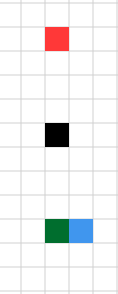
\includegraphics[height=5cm]{Bilder/pathfinding_procedure_1.png}
				\caption{\\ 1. Feld wird durchlaufen} 
				\label{pic:pathfinding_procedure_1}
			\end{minipage}
			\begin{minipage}{0.5\textwidth}
				\centering
				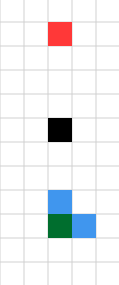
\includegraphics[height=5cm]{Bilder/pathfinding_procedure_2.png}
				\caption{\\ 2. Feld wird durchlaufen} 
				\label{pic:pathfinding_procedure_2}
			\end{minipage}
		\newline
			\begin{minipage}{0.5\textwidth}
				\centering
				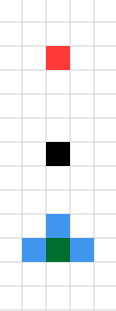
\includegraphics[height=5cm]{Bilder/pathfinding_procedure_3.png}
				\caption{\\ 3. Feld wird durchlaufen} 
				\label{pic:pathfinding_procedure_3}
			\end{minipage}
			\begin{minipage}{0.5\textwidth}
				\centering
				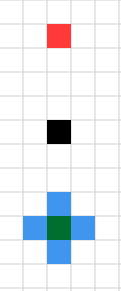
\includegraphics[height=5cm]{Bilder/pathfinding_procedure_4.png}
				\caption{\\ 4. Feld wird durchlaufen}
				\label{pic:pathfinding_procedure_4}
			\end{minipage}
		\end{figure}
		
		
		%evtl \newpage
		Dies wird in der unteren Abbildung verdeutlicht. Grün repräsentiert den Startpunkt, Rot den Endpunkt. Schwarz repräsentiert ein nicht passierbares Feld und blaue Felder sind von dem Suchalgorithmus bereits besucht worden. 
		Die dargestellte Suchart stellt den \textbf{Breadth-first Search Algorithmus} dar, welche zur oben gegebenen Beschreibung passt. Dabei handelt es sich um einen einfachen Wegfindungsalgorithmus.
		
		\begin{figure}[H]
			\begin{minipage}{0.5\textwidth}
				\centering
				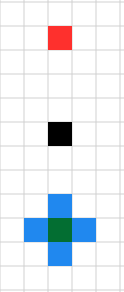
\includegraphics[height=5cm]{Bilder/pathfinding_tiefe1.png}
				\caption{Besuchte Felder nachdem die \\ Tiefe 1 durchlaufen wurde} %\parencite{flora85}}
				\label{pic:pathtiefe1}
			\end{minipage}
			\begin{minipage}{0.5\textwidth}
				\centering
				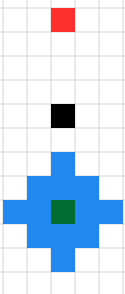
\includegraphics[height=5cm]{Bilder/pathfinding_tiefe2.png}
				\caption{Besuchte Felder nachdem die \\ Tiefe 2 durchlaufen wurde} %\parencite{northFlora190105}}
				\label{pic:pathtiefe2}
			\end{minipage}
		\end{figure}	
	
		Zur Verbesserung der Effizienz nutzen manche Algorithmen weitere Algorithmen, die Schätzalgorithmen, welche man auch Heuristik nennt, die Einfluss darauf nehmen, welche Felder als nächstes besucht werden. Felder, welche in Richtung des Ziels zeigen bzw. sehr wahrscheinlich dorthin führen, werden bevorzugt durchlaufen, Felder, welche vom Ziel weg zeigen, werden hingegen seltener Besucht. Dazu misst der Algorithmus nicht nur die Distanz(Kosten) bis zu einem Punkt, um zu berechnen, ob es sich lohnt, von diesem aus weiter zu suchen, sondern auch die Distanz zum Ziel. Mathematisch kann man dies als zusammengesetzte Funktion verstehen.
		\begin{equation}
			f(x) = g(x) + h(x)
		\end{equation}
		
		Hierbei stellt $g(x)$ die Funktion dar, welche die Kosten(Distanz) vom Startpunkt bis zu einem Punkt $x$ berechnet. $h(x)$ beschreibt die vermutete Distanz von $x$ bis zum Zielpunkt. Beide Ergebnisse zusammen ergeben einen Wert, welcher die Kosten über einen Punkt $x$ zum Zielpunkt errechnet. Dies wird für viele Punkte $x$ berechnet, wobei der nächste Schritt von dem Punkt ausgeht, welcher den niedrigsten Wert (also die geringste, errechnete Distanz) hat.
		Diese Algorithmen sind für viele Verwendungszwecke sehr effizient. Heuristik nutzende Wegfindungsalgorithmen können unter Umständen nachteilig sein, wenn diese in Labyrinthen eingesetzt werden, welche eine hohe Komplexität aufweisen, da Sackgassen, welche nur durch eine Wand vom Ziel getrennt werden, meist durchsucht werden, obwohl sie im Endeffekt nicht Zielführend sind.
		
		\begin{figure}[H]
			\centering
			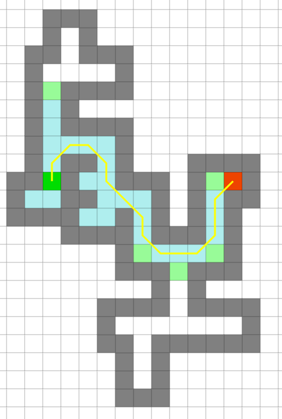
\includegraphics[height=5cm]{Bilder/pathfinding_laby_heu.png}
			\caption{Wegfindung eines Algorithmus mit Heuristik} 
			\label{pic:pathlabheu}
		\end{figure}
		
		\subsection{Costmap}
		{
			Eine gemessene Karte wird zur Navigation zu einer Coastmap umgewandelt. Diese enthält Daten, welche während  der Kartenerstellung nicht angezeigt, trotzdem aber gesammelt werden. Im Falle einer Coastmap wird nicht nur betrachtet, ob ein Punkt besetzt oder frei ist, sondern auch, wie schwierig es ist, gewisses Terrain zu überqueren. Zwar sind diese Daten in einer ebenen Fläche relativ irrelevant, vor allem aber bei hügeligem Boden sind diese interessanter, weshalb ich dies hier erwähnen wollte. Dies weiteren erhalten Hindernisse einen Radius, welcher von dem Roboter tendenziell vermieden werden sollte, da Kollisionen, u.a. aufgrund der Objektform oder ungenauer Messdaten möglich sein Könnte.
		}
		
		\subsection{Positionierung auf einer Karte}
		{
			Zwar hat der Roboter nun eine Karte seiner Umgebung, jedoch fehlt dem Roboter noch sein genauer Standpunkt, da er sich auf irgendeinem Punkt in der Karte befinden könnte. Um nun den genauen Standpunkt zu finden, nutzt man die Monte-Carlo-Lokalisation. Dafür wird die Karte der Umgebung, sowie die Sensordaten, benötigt. Anfangs ist es gleich wahrscheinlich, dass der Roboter sich in jeglicher Stelle auf der Karte befindet. Nun werden die gemessenen Sensorpunkte und die Karte der Umgebung übereinander gelegt. Stimmen Hindernisse, welche durch die Karte in der Nähe sind, sowie gemessene Sensordaten der realen Welt überein, so ist es wahrscheinlich, dass sich der Roboter an dieser Stelle in der Karte befindet. Misst der Turtlebot beispielsweise einen Runden Gegenstand vor sich und in einer Position auf der Karte ist in gleicher Distanz eine Runde Säule vor dem Roboter, so ist es wahrscheinlich, dass der Roboter sich in dieser Position befindet. In der beigefügten Abbildung, wird das vergleichen von Sensordaten und Karte deutlich.
			\begin{figure}[H]
				\centering
				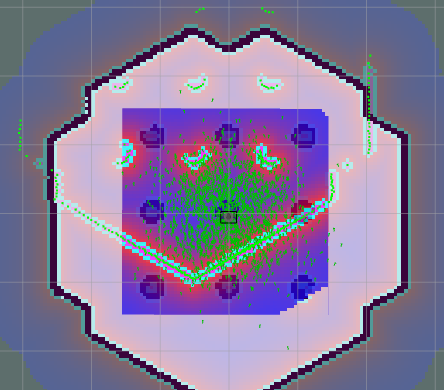
\includegraphics[height=5cm]{Bilder/coastmap_monte_carlo_example.png}
				\caption{Coastmap mit Sensordaten} 
				\label{pic:coastmontecarlo}
			\end{figure}
		In der Abbildung wird deutlich, dass der Roboter auf der gegebenen Karte (Hintergrund) mittig platziert wird. Gleichzeitig misst der LiDAR-Sensor auch Hindernisse, welche wiederum eine neue Karte der Umgebung bilden. Diese Hindernisse sind Hell im Vordergrund zu sehen. Man erkennt, dass diese nicht übereinander liegen und der Roboter deshalb noch nicht korrekt positioniert ist. In Wirklichkeit werden Daten aus der unteren linken Ecke der Karte gemessen. Dadurch werden Positionen in dieser Umgebung sehr wahrscheinlich. Damit der Roboter bei vielen ähnlichen Stellen, was hier nicht der Fall ist, trotzdem korrekt positioniert ist, wird der Roboter zwischen verschiedenen LiDAR-Messungen bewegt. Während der Bewegungen wird errechnet, wo der Roboter sich, ausgehend von den Ursprünglichen Vermutungen der Position, befindet. Stimmen auch die neuen Messungen mit der Karte überein, so wird eine Position immer wahrscheinlich, bis der Roboter schlussendlich, sicher positioniert werden kann, da Sensordaten und Karte übereinstimmen. im Falle anderer Roboter können neben LiDAR-Sensoren auch andere Sensordaten verwendet werden.
		}
		\subsection{Die Move-Base} %https://www.researchgate.net/publication/253239158_ROSoClingo_A_ROS_package_for_ASP-based_robot_control
		{
			Um den Roboter nun zu einem Ziel zu navigieren, wird das move\textunderscore base-Package verwendet. Dieses steuert die Navigation des Roboters, sowie den Pfad, welchem der Roboter folgen soll. Es besteht aus mehreren Nodes (in der Abbildung oval dargestellt).  Dazu abonniert diese Nodes verschiedene Topics. Dazu gehören Sensordaten (z.B. sensor\textunderscore msgs/LaserScan für die Daten des LiDAR-Sensors), Odometriedaten und eine Karte. Die Karte wird durch einen Kartenserver bereitgestellt, welcher, als Node, diese Karte veröffentlicht, sodass jegliche Programme darauf zugreifen können. Dafür muss die Karte jedoch als Bild vorliegen, weshalb die Karte nach vollendeter Kartierung des Labyrinth auf einem Datenträger, meist die Festplatte eines über Wifi mit dem Turtlebot verbundenen Computers, gespeichert werden muss. Die gespeicherte Karte kann daraufhin von dem Karten-Server geöffnet werden. Dieses System sorgt gleichzeitig dafür, dass man eine Umgebung zur Navigation nicht notwendigerweise erneut kartieren muss, sollte schon eine Karte existieren. Im Anwendungsfall ist dies auch praktisch. Staubsageroboter müssen daher beispielsweise nicht jedes mal erneut eine komplette Karte eines Hauses erstellen.
		\begin{figure}[H]
			\centering
			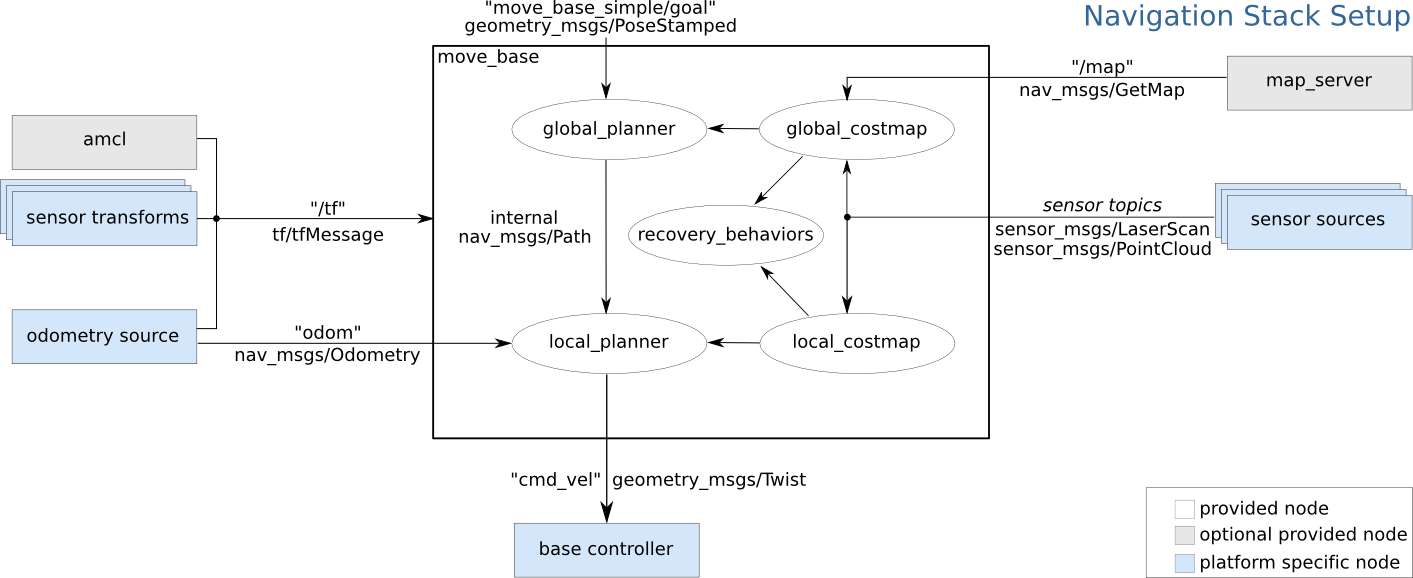
\includegraphics[height=8cm]{Bilder/overview_move_base.png}
			\caption{Das move\textunderscore base-Package \\
			\parencite{movebasenodeoverview}} 
			\label{pic:overviewmovebase}
		\end{figure}
			
			 Nachdem der Roboter nun auf der durch den Kartenserver bereitgestellten Karte verordnet ist, muss dem Roboter ein Navigationsziel gegeben werden.
			 Dazu gibt es mehrere Möglichkeiten. Das Programm Rviz ermöglicht es, wie bereits erwähnt, die Karte zu visualisieren. Gleichzeitig hat dies den Nebeneffekt, dass man durch das Programm bestimmen kann, welche Koordinaten ein Punkt auf der Karte hat, indem man die Maus auf diesen Bewegt. Rviz ermöglicht es sogar, direkt im Programm ein Navigationsziel festzulegen, was jedoch teilweise von dem Roboter nicht akzeptiert wird, weshalb ich ein Skript nutze, um die Koordinaten des Zielpunktes, welche ich in Rviz ablesen kann, an das move\textunderscore base-Package zu übertragen.
			 Dafür wird folgendes Skript verwendet, in welchem der Roboter sich beispielhaft zu dem Punkt $P(3|2)$ bewegen soll:
			 \newline  %https://answers.ros.org/question/80646/python-sending-goals-to-the-navigation-stack/
			
			\lstset{
				breaklines = true,
				frame = single,
				numbers = none
			}
\begin{lstlisting} [language=Python]
	01 import actionlib
	02 import rospy
	03 from move_base_msgs.msg import MoveBaseAction, MoveBaseGoal,   MoveBaseFeedback, MoveBaseResult
			 	
	04 rospy.init_node("nav_goal_sender")
			 	
	05 client = actionlib.SimpleActionClient("/move_base", MoveBaseAction)
	06 client.wait_for_server()
			 	
	07 goal = MoveBaseGoal()
	08 goal.target_pose.header.frame_id = 'map' 
	09 goal.target_pose.pose.position.x = 3
	10 goal.target_pose.pose.position.y = 2
	11 goal.target_pose.pose.orientation.z = 0
	12 goal.target_pose.pose.orientation.w = 0.5
			 	
	13 client.send_goal(goal)
	14 client.wait_for_result()
			 	
\end{lstlisting}
		 	Nun erläutere ich das Programm kurz Stück für Stück.
		 	Mit Hilfe der \textbf{import}-Befehle werden Bibliotheken eingebunden (Z. 1-3), welche Funktionalitäten für das Programm beinhalten, welche benötigt werden. Dazu zählt z.B: \textbf{rospy} (Z.2), welches eine Interaktion mit dem ROS-Betriebssystem ermöglicht, sowie verschiedene Klassen  \footcite{Programmierung: Ansammmlung von Funktionen (eines Aufgabenbereiches)}, welche mit dem move\textunderscore base-Package zusammenhängen (Z.3).
		 	
		 	Daraufhin wird eine Node-initiiert, deren einzige Funktion ist, ein Navigatinsziel auszusenden. Die Node erhält den Namen "\textit{nav\textunderscore goal\textunderscore sender}" (Z.4).
		 	
		 	In den nächsten zwei Zeilen wird ein "Action-Client" \space initiiert. Dies ist eine Klasse, welche es ermöglicht, eine Action an einen Service auszusenden. Diese Art des Datenaustausches wurde in Abschnitt 1.3.2- "Services" ausgeführt. Die Initiierung bedeutet vereinfacht gesagt, dass alles vorbereitet wird, sodass ein Befehl an den Service des move\textunderscore base-Packetes gesendet werden kann (Z.5f.).
		 	
		 	In den nachfolgenden sechs Zeilen (Z.7-12) werden die Parameter gesetzt, welche die Position, zu welcher Navigiert werden soll, bestimmen. Hier ist die z-Koordinate irrelevant, da der Roboter sich nicht nach oben/unten bewegen kann. Die x Koordinate (Z.9) wird gleich drei gesetzt. Die y-Koordinate gleich 2 (Z.10). In Zeile 11 wird die Richtung, in welche der Roboter am Ende schauen soll, festgesetzt.
		 	
		 	In Zeile 13 wird eine Action, also der Befehl mit den eingestellten Parametern, hier sind dies die Koordinaten, an den move\textunderscore base Service geschickt, welcher daraufhin zu diesem Ziel navigiert.
		 	
		 	
			
		}
	}
}